\documentclass[a4paper]{article}
\usepackage[utf8]{inputenc}
\usepackage[T1]{fontenc}
\usepackage[french]{babel}
\usepackage{graphicx}
\usepackage{caption}
\usepackage{subcaption}
\usepackage{hyperref}

\begin{document}



\section{Présentation de l'environnement PyGame}

\subsection{Intérêt d'utilisation de la bibliothèque PyGame}

\textbf{PyGame} est une bibliothèque libre multi-plateforme qui facilite le développement de jeux vidéo en temps réel avec le langage de programmation Python, langage utilisé dans le cadre de ce projet.
Cette bibliothèque permet principalement de développer une interface graphique par l'intermédiaire du langage Python.

\begin{figure}[!h] 
\centering
\fbox{
\includegraphics[scale=0.4]{0.png}}
\caption{Logo PyGame} 
\end{figure} 

Il est intéressant de se demander pourquoi avoir choisi une telle bibliothèque pour le développement d'une interface graphique.

\vspace{0.3cm}

Celle-ci possède plusieurs points forts qui peuvent être énumérés ci-dessous :

\begin{itemize}

   \item Une portabilité sur divers systèmes d'exploitation


   \item Facilité d'utilisation avec la multitude de fonctionnalités offerte par une telle libraire

   \item Construction sur la bibliothèque logicielle libre Simple DirectMedia Layer (SDL) qui supporte plusieurs OS

   \item Gestion de l'affichage vidéo, de périphériques communs avec le clavier et la souris,  de l'audio numérique


\end{itemize}



\subsection{Exemples d'utilisation}

Pour se familiariser avec les fonctionnalités proposées par la bibliothèque PyGame, il peut être intéressant de pouvoir découvrir ce qu'il en est à travers différents exemples d'utilisation qui seront présentés à la suite.

\vspace{0.5cm}



Le programme 1 permet de construire une fenêtre d'affichage donnée en spécifiant ses dimensions (largeur,hauteur) exprimées en pixels. Après exécution du programme, une fenêtre d'affichage noire se lance et change de couleur après appui sur une touche de clavier par l'utilisateur, la couleur de la fenêtre d'affichage bascule du noir vers le blanc et vice-versa.
Le code source et les résultats obtenus sont illustrés sur la page suivante.

\newpage

\begin{figure}[h!]
\centering
\fbox{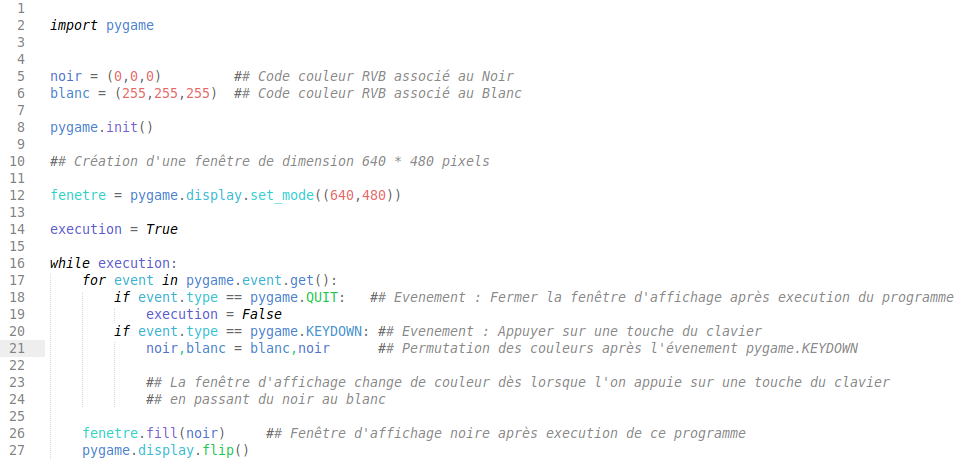
\includegraphics[scale=0.35]{prgm1.png}}
\caption{Code source du programme 1}
\end{figure}



\begin{figure}[h!]
   \begin{minipage}[b]{0.40\linewidth}
      \centering 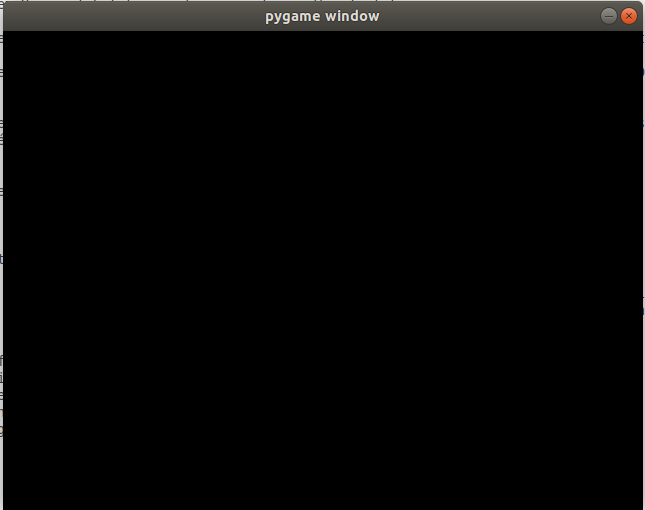
\includegraphics[width=4.8cm,scale=1.8]{f1.png}
      \caption{Fenêtre d'affichage avant l'appui sur une touche de clavier}
   \end{minipage}\hfill
   \begin{minipage}[b]{0.40\linewidth}   
      \centering 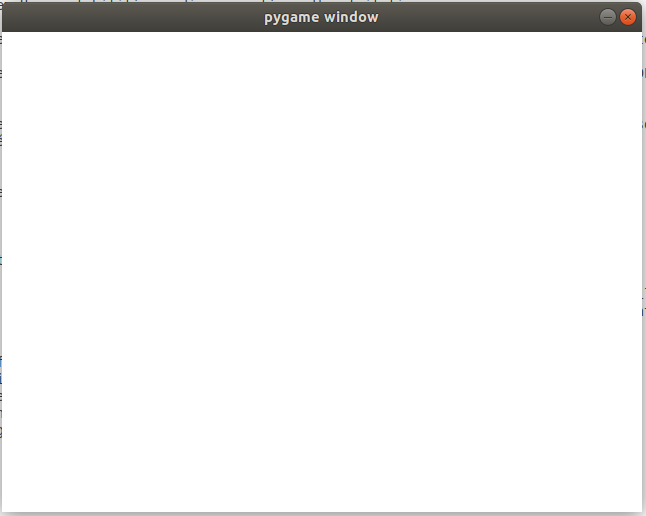
\includegraphics[width=4.8cm,scale=1.8]{f2.png}
      \caption{Fenêtre d'affichage après l'appui sur une touche de clavier}
   \end{minipage}

   \end{figure}


Intéressons nous à présent à la construction de figures géométriques, la bibliothèque PyGame compte une multitude de fonctions
permettant de réaliser des figures géométriques à partir d'une fenêtre d'affichage. 
L'exemple ci-dessous concerne la construction d'un cercle avec un rayon spécifié, le code source correspondant se base en partie de celui du premier programme.


\begin{figure}[h!]
   \begin{minipage}[b]{0.10\linewidth}
      \centering 
      \fbox{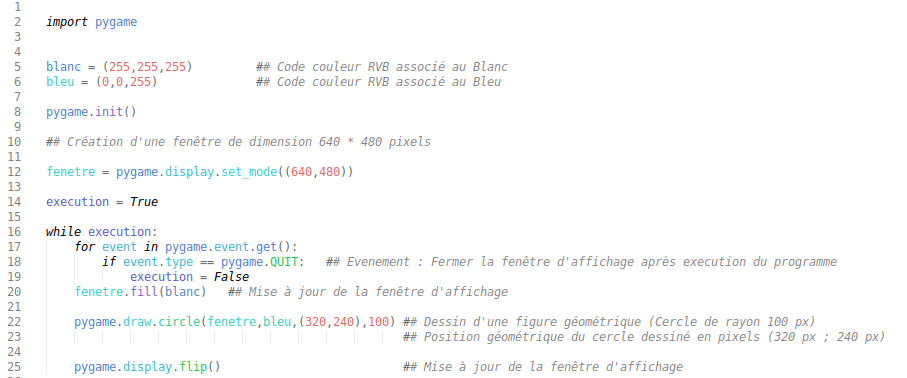
\includegraphics[scale=0.3]{prgm2.png}}
 
   \end{minipage}\hfill
   \begin{minipage}[b]{0.10\linewidth}   
      \centering 
      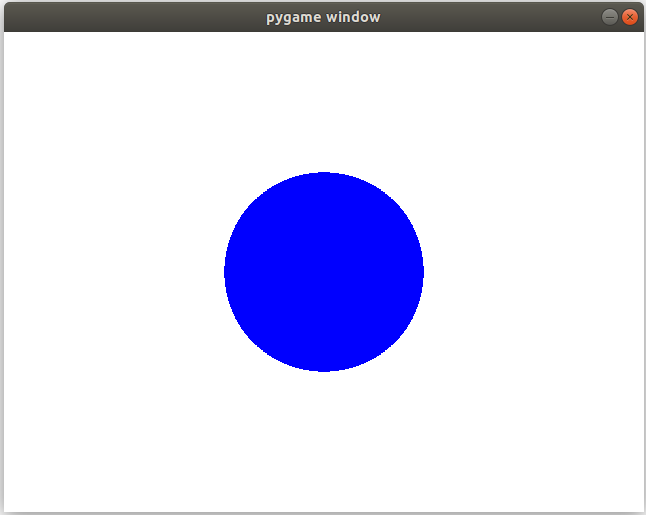
\includegraphics[scale=0.2]{img2.png}
      
  
   \end{minipage}

   \end{figure}


\newpage

Le troisième et dernier exemple d'utilisation va concerner la création de boutons.
Cet exemple consiste à créer une suite de boutons ayant une forme géométrique donnée, après un clic sur un des boutons une
animation est déclenchée (disparition du bouton / changement de couleur d'un bouton).

\vspace{0.3cm}

\centering
\fbox{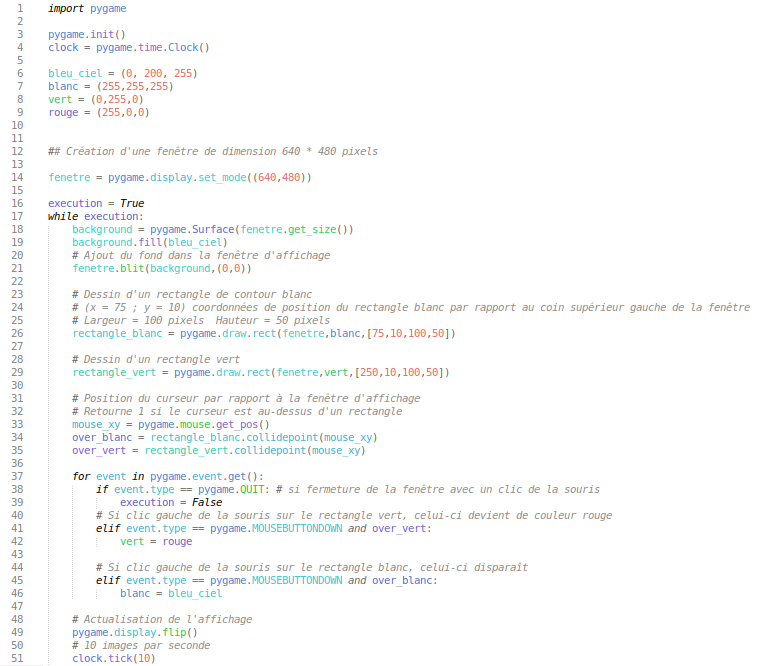
\includegraphics[scale=0.42]{prgm3.png}}


\begin{figure}[h!]
   \begin{minipage}[l]{0.50\linewidth}
      \centering 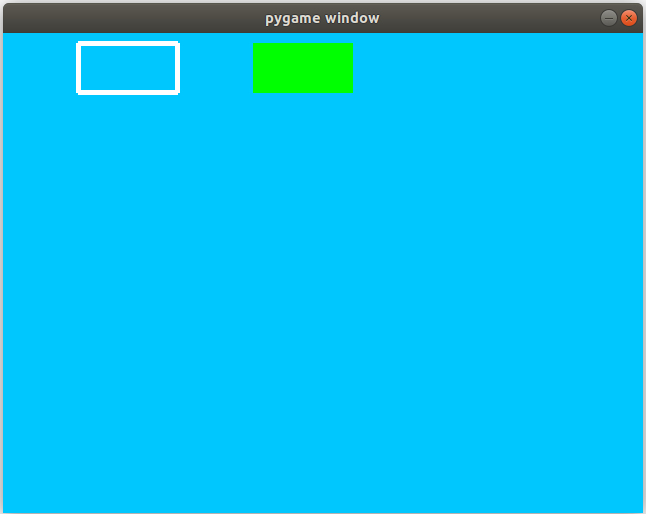
\includegraphics[scale=0.20]{img3.png}
      \caption{Fenêtre d'affichage}
 
   \end{minipage}\hfill
   \begin{minipage}[l]{0.50\linewidth}   
      \centering 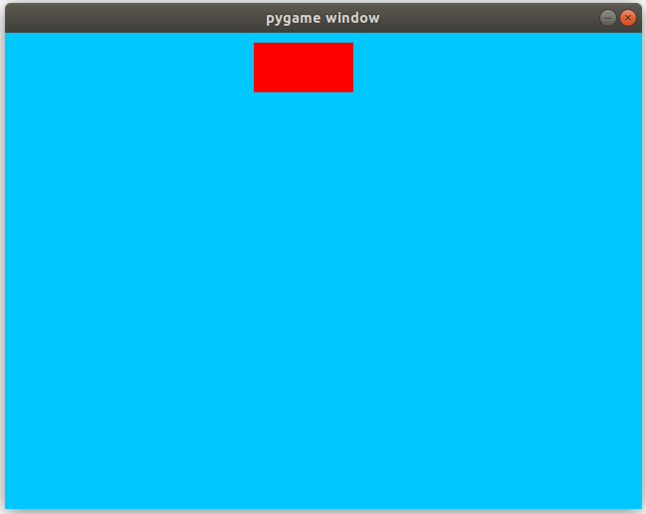
\includegraphics[scale=0.20]{img4.png}
      \caption{Animations après clic}
  
   \end{minipage}

   \end{figure}


La bibliothèque PyGame propose davantage de fonctionnalités, de nombreux tutoriels sont présents afin de se familiariser avec cet environnement.
La documentation de PyGame est consultable via le lien ci-dessous : \url{https://www.pygame.org/docs/}

\newpage

\subsection{Interface graphique proposée pour le Puissance 4}

Il est à présent important de se focaliser sur le projet concerné, il sera question ici de présenter et d'expliquer le développement de l'interface graphique proposée pour le jeu du Puissance 4.

Premièrement, il a été nécessaire de définir correctement l'environnement de jeu. Le code ci-dessous décrit la définition des paramètres géométriques sur l'environnement concerné.
Il a été question de fixer une taille pour la grille de jeu adaptée pour une dimension 6 * 7, cette taille a été choisie de manière à ce que cela soit adaptée avec la dimension souhaitée.

Il a fallu de plus, définir le rayon du cercle autrement dit l'emplacement nécessaire à l'insertion des jetons. Cela a été défini en tenant compte de la propriété géométrique d'une case (rectangle avec un cercle inscrit).

Pour rendre un tel environnement jouable, il a fallu ajouter à cela des jetons de jeu (jaune et rouge), des pions utilisées pour des fonctions prochaines.

La fenêtre de jeu doit être adaptée avec le dimensionnement de la grille, d'où la définition de largeur et de hauteur sur le code ci-dessous.



\begin{figure}[!h] 
\centering
\fbox{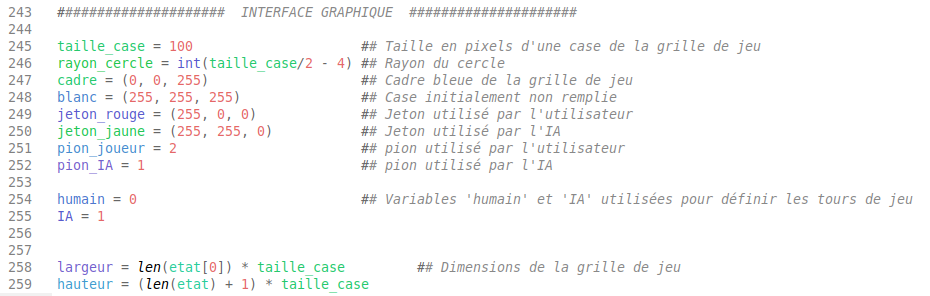
\includegraphics[scale=0.4]{img5.png}}
\caption{Spécifications Géométriques} 
\end{figure} 

Une fois avoir présenté l'environnement de jeu, il est maintenant important d'aborder les fonctions nécessaires à l'évolution du jeu.

La première fonction\textit{inserer jeton} prend comme paramètres :
 
 \begin{itemize}
 \item Un état du jeu qui est la grille
 \item i étant l'indice de ligne de la case utilisée pour l'insertion d'un jeton
 \item j étant l'indice de colonne de la case pour laquelle on veut insérer un jeton
 \end{itemize}

Celle-ci effectue au cours du jeu les insertions de jeton pour l'humain et l'IA, on retrouvera cette fonction dans la boucle de jeu qui sera abordée plus tard.

La fonction suivante \textit{emplacementValide} prend comme paramètres l'état de jeu et l'indice de la colonne de la case souhaitée pour effectuer l'insertion d'un jeton de jeu.
L'emplacement est valide lorsqu'un jeton occupe la postion la plus basse possible sur une colonne donnée. Cette fonction renvoie un booléen pour indiquer si l'insertion est permise ou non.

\newpage

La troisième et dernière fonction de jeu \textit{rangeeSuivante} prend les mêmes paramètres que la fonction précédente. En revanche, celle-ci renvoie l'indice le plus grand de la ligne d'un état de jeu pas encore complétée de jetons de jeu.
Exemple, si la dernière rangée est complétée de jetons de jeu il suffira de rechercher l'indice le plus grand de la rangée non encore complétée, étant donné qu'un jeton à insérer doit occuper la position la plus basse possible sur une colonne précise de la grille de jeu.


\begin{figure}[h!]
      \centering 
      \fbox{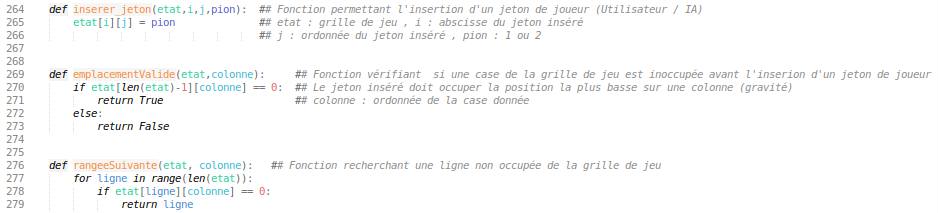
\includegraphics[scale=0.46]{img6.png}}
      \caption{Fonctions de jeu}
 \end{figure}


La fonction suivante est l'une des fonctions principales pour le développpement de l'interface graphique.
Celle-ci va s'occuper de l'affichage de la grille de jeu, la grille de jeu se construit de manière itérative. 
En parcourant toute la grille qu'on peut assimiler à une matrice, les cases se construisent progressivement. Chaque case est représentée par un rectangle avec des dimensions choisies (largeur,hauteur) et des coordonées de position (x;y) par rapport à la grille de jeu. Chaque rectangle contient un cercle ayant un rayon défini et aussi des coordonées de position (x,y) par rapport à la grille de jeu.

Les dimensions proposées dans le code ci-dessous ont été choisies de manière à ce que cela s'adapte au mieux aux dimensions de la grille de jeu.

Elle se construit ainsi progressivement dès lorsque des insertions de jetons de jeu ont été effectuées, cette fonction fera l'objet de plusieurs appels car à chaque insertion de jetons il est nécessaire de mettre à jour l'affichage de la grille de jeu.

\vspace{0.5cm}


\begin{figure}[h!]
      \centering 
      \fbox{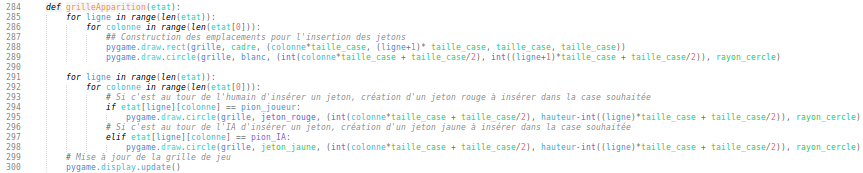
\includegraphics[scale=0.5]{img7.png}}
      \caption{Création de la grille de jeu}

\end{figure}

\newpage

La dernière étape ayant permis la réalisation de l'interface graphique est la fonction jeu().
Cette fonction peut se décomposer en plusieurs phases :
\vspace{0.3cm}
\begin{itemize}

   \item Gestion des tours de jeu
   \item Insertion d'un jeton de jeu dans le cas où c'est au tour de l'utilisateur de débuter la partie
   \item Insertion d'un jeton de jeu dans le cas où c'est au tour de l'IA de commencer
   \item Détermination de l'état final du jeu (Victoire de l'utilisateur / Victoire de l'IA / Match nul)

\end{itemize}

Les différentes phases sont décrites par les deux illustrations qui suivent.

\begin{figure}[h!]
      \centering 
      \fbox{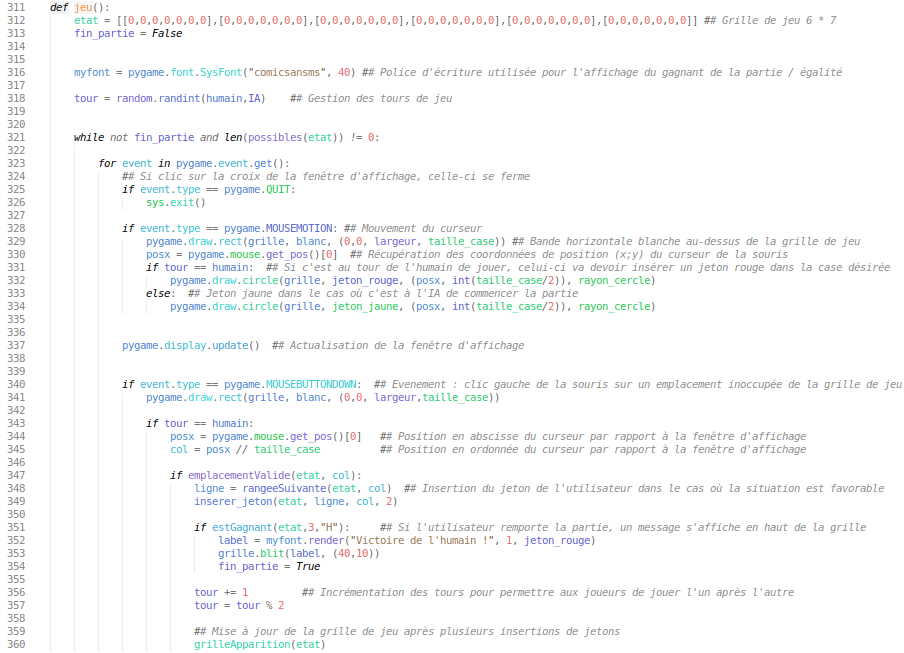
\includegraphics[scale=0.45]{img8.png}}
      \caption{Partie 1 de la fonction jeu()}
\end{figure}

\newpage

\begin{figure}[h!]
      \centering 
      \fbox{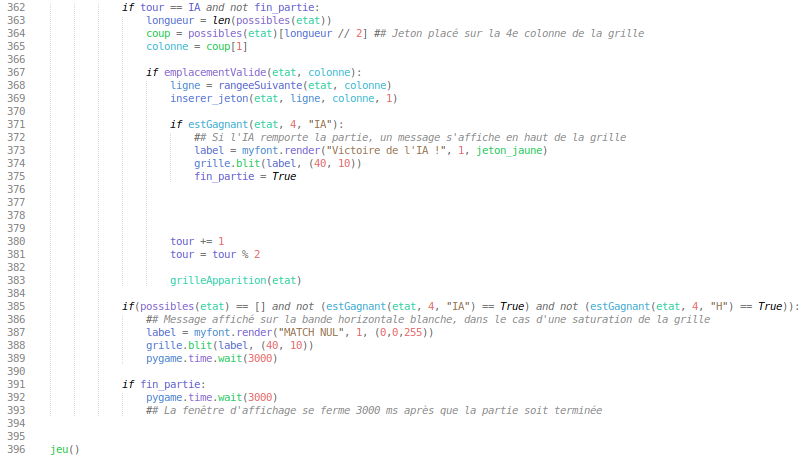
\includegraphics[scale=0.45]{img9.png}}
      \caption{Partie 2 de la fonction jeu()}

\end{figure}



\subsection{Tests effectués sur une grille traditionnelle 6 * 7}



\begin{figure}[h!]
   \begin{minipage}[c]{0.60\linewidth}
      \centering 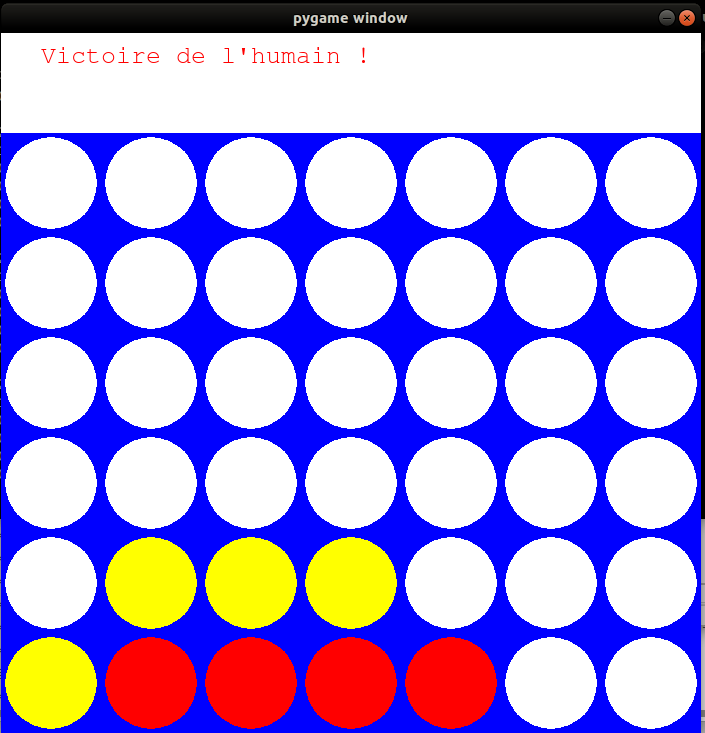
\includegraphics[scale=0.15]{humanv.png}
      \caption{Victoire de l'utilisateur}
 
   \end{minipage}\hfill
   \begin{minipage}[c]{0.60\linewidth}   
      \centering 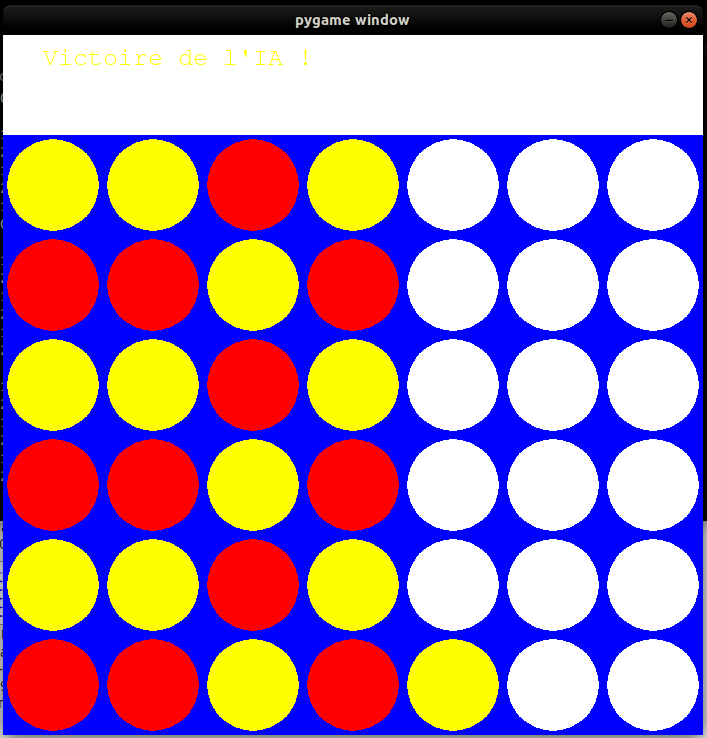
\includegraphics[scale=0.15]{iav.png}
      \caption{Victoire de l'IA}
  
   \end{minipage}\hfill
   \begin{minipage}[c]{0.60\linewidth}   
      \centering 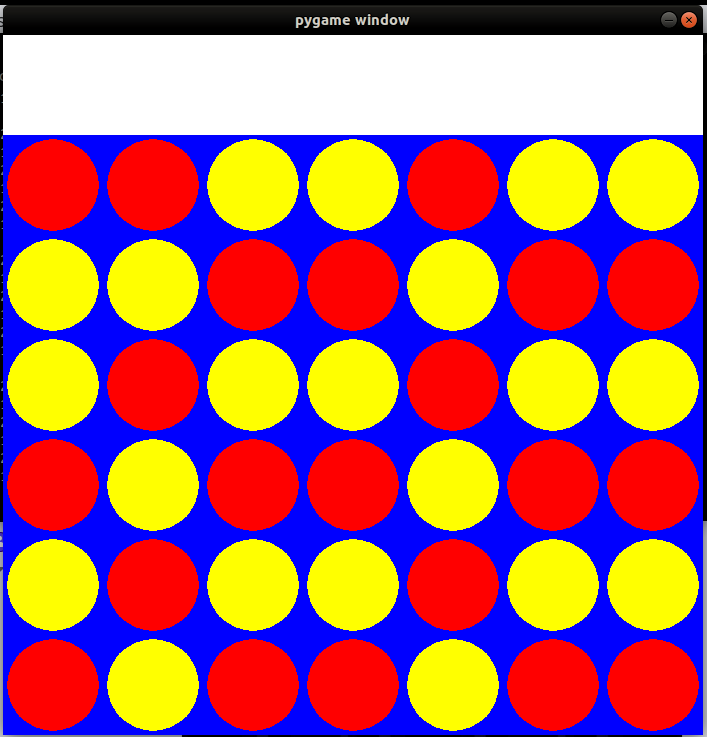
\includegraphics[scale=0.15]{draw.png}
      \caption{Saturation de la grille}

      \end{minipage}


   \end{figure}




\end{document}